\section{Introduction}

This document describes client requirements and system 
requirements for a SQUID magnetometer program that will be designed and 
implemented as a software engineering student project at University of 
Helsinki at the Computer Science Department. The client is the Department 
of Geophysics.

This document serves as a contract between client and us about the implemented functions of the program. Particulary the 
requirements part of this document describes them.

Expected readership of this document here..


\subsection{Glossary}

Technical terms here..



\section{Overview}

Department of Geophysics uses a magnetometer that works in SQUID (superconducting quantum interference device) 
principle to measure magnetization of minerals and rocks. Magnetometer is controlled by a computer software 
that controls and reads electric components that control the device itself.

The use of the present magnetometer software is complicated and unnecessarily burdens the users work memory 
with complicated work phases and divergent operation in different use cases. The device is now controlled with 
two various program. Functions of those two program can be combined to one. Now the programs are hard to learn and 
teach which restricts the group of users.

User of the device must know clearly what is the state of it and which operation is being performed at the 
moment. The device is delicate and expensive, so a misfunction of it must be noticed early to prevent damage. 
For example faulty state of demagnetizer can damage the device if it's not shut down manually in time.
 
Device and program are used to carry out long, several stages involving measurement sequeances. It's 
important that these sequences can be performed flexibly and fast. User must be able to follow the 
measuring procedure and to stop and modify sequence if there is unexpected changes in results.

Further process and analyze of the results occurs in various other programs which use a standard file format. 
So the new program has to export these formats.

\section{Use cases}

% super-makrot use caseille; huomaa ett� \uctitle aloittaa ja \ucend lopettaa, muuten tulee ongelma
\newcommand{\ucsecdesc}[1]{\textit{#1}\\}
\newcommand{\uctitle}[1]{\refstepcounter{ucnum}\textbf{UC\arabic{ucnum}: #1}\\\begin{tabular}{p{3cm}p{11cm}}}
\newcommand{\ucnote}[1]{\multicolumn{2}{p{14cm}}{[\textsc{#1}]}\\}
\newcommand{\ucnotein}[1]{[\textsc{#1}]}
\newcommand{\ucscenario}[1]{\stepcounter{ucsce}\textbf{Scenario \alph{ucsce}} & #1\\}
\newcommand{\ucpre}[1]{\textbf{Precondition} & #1\\}
\newcommand{\ucpost}[1]{\textbf{Postcondition} & #1\\}
\newcommand{\ucerror}[1]{\textbf{Error condition} & #1\\}
\newcommand{\ucgd}[1]{\textbf{Goal-derived} & #1\\}
\newcommand{\ucreq}[1]{\textbf{Requirements} & #1\\}
\newcommand{\ucend}[0]{\end{tabular}\\}
\newcounter{ucnum}
\newcounter{ucsce}[ucnum]
\hbadness=10000 % est�mm� ihme "underfull \hbox (badness 10000)" -varoitukset (ei hajua mist� tulevat)

Describes planned use cases for the program. Use cases are derived from user interface prototype and requirements. All use cases are perfomed by any ordinary user and in program main screen. A simplified use case diagram is presented in Figure~\ref{fig:usecases}.

\begin{figure}
\begin{center}
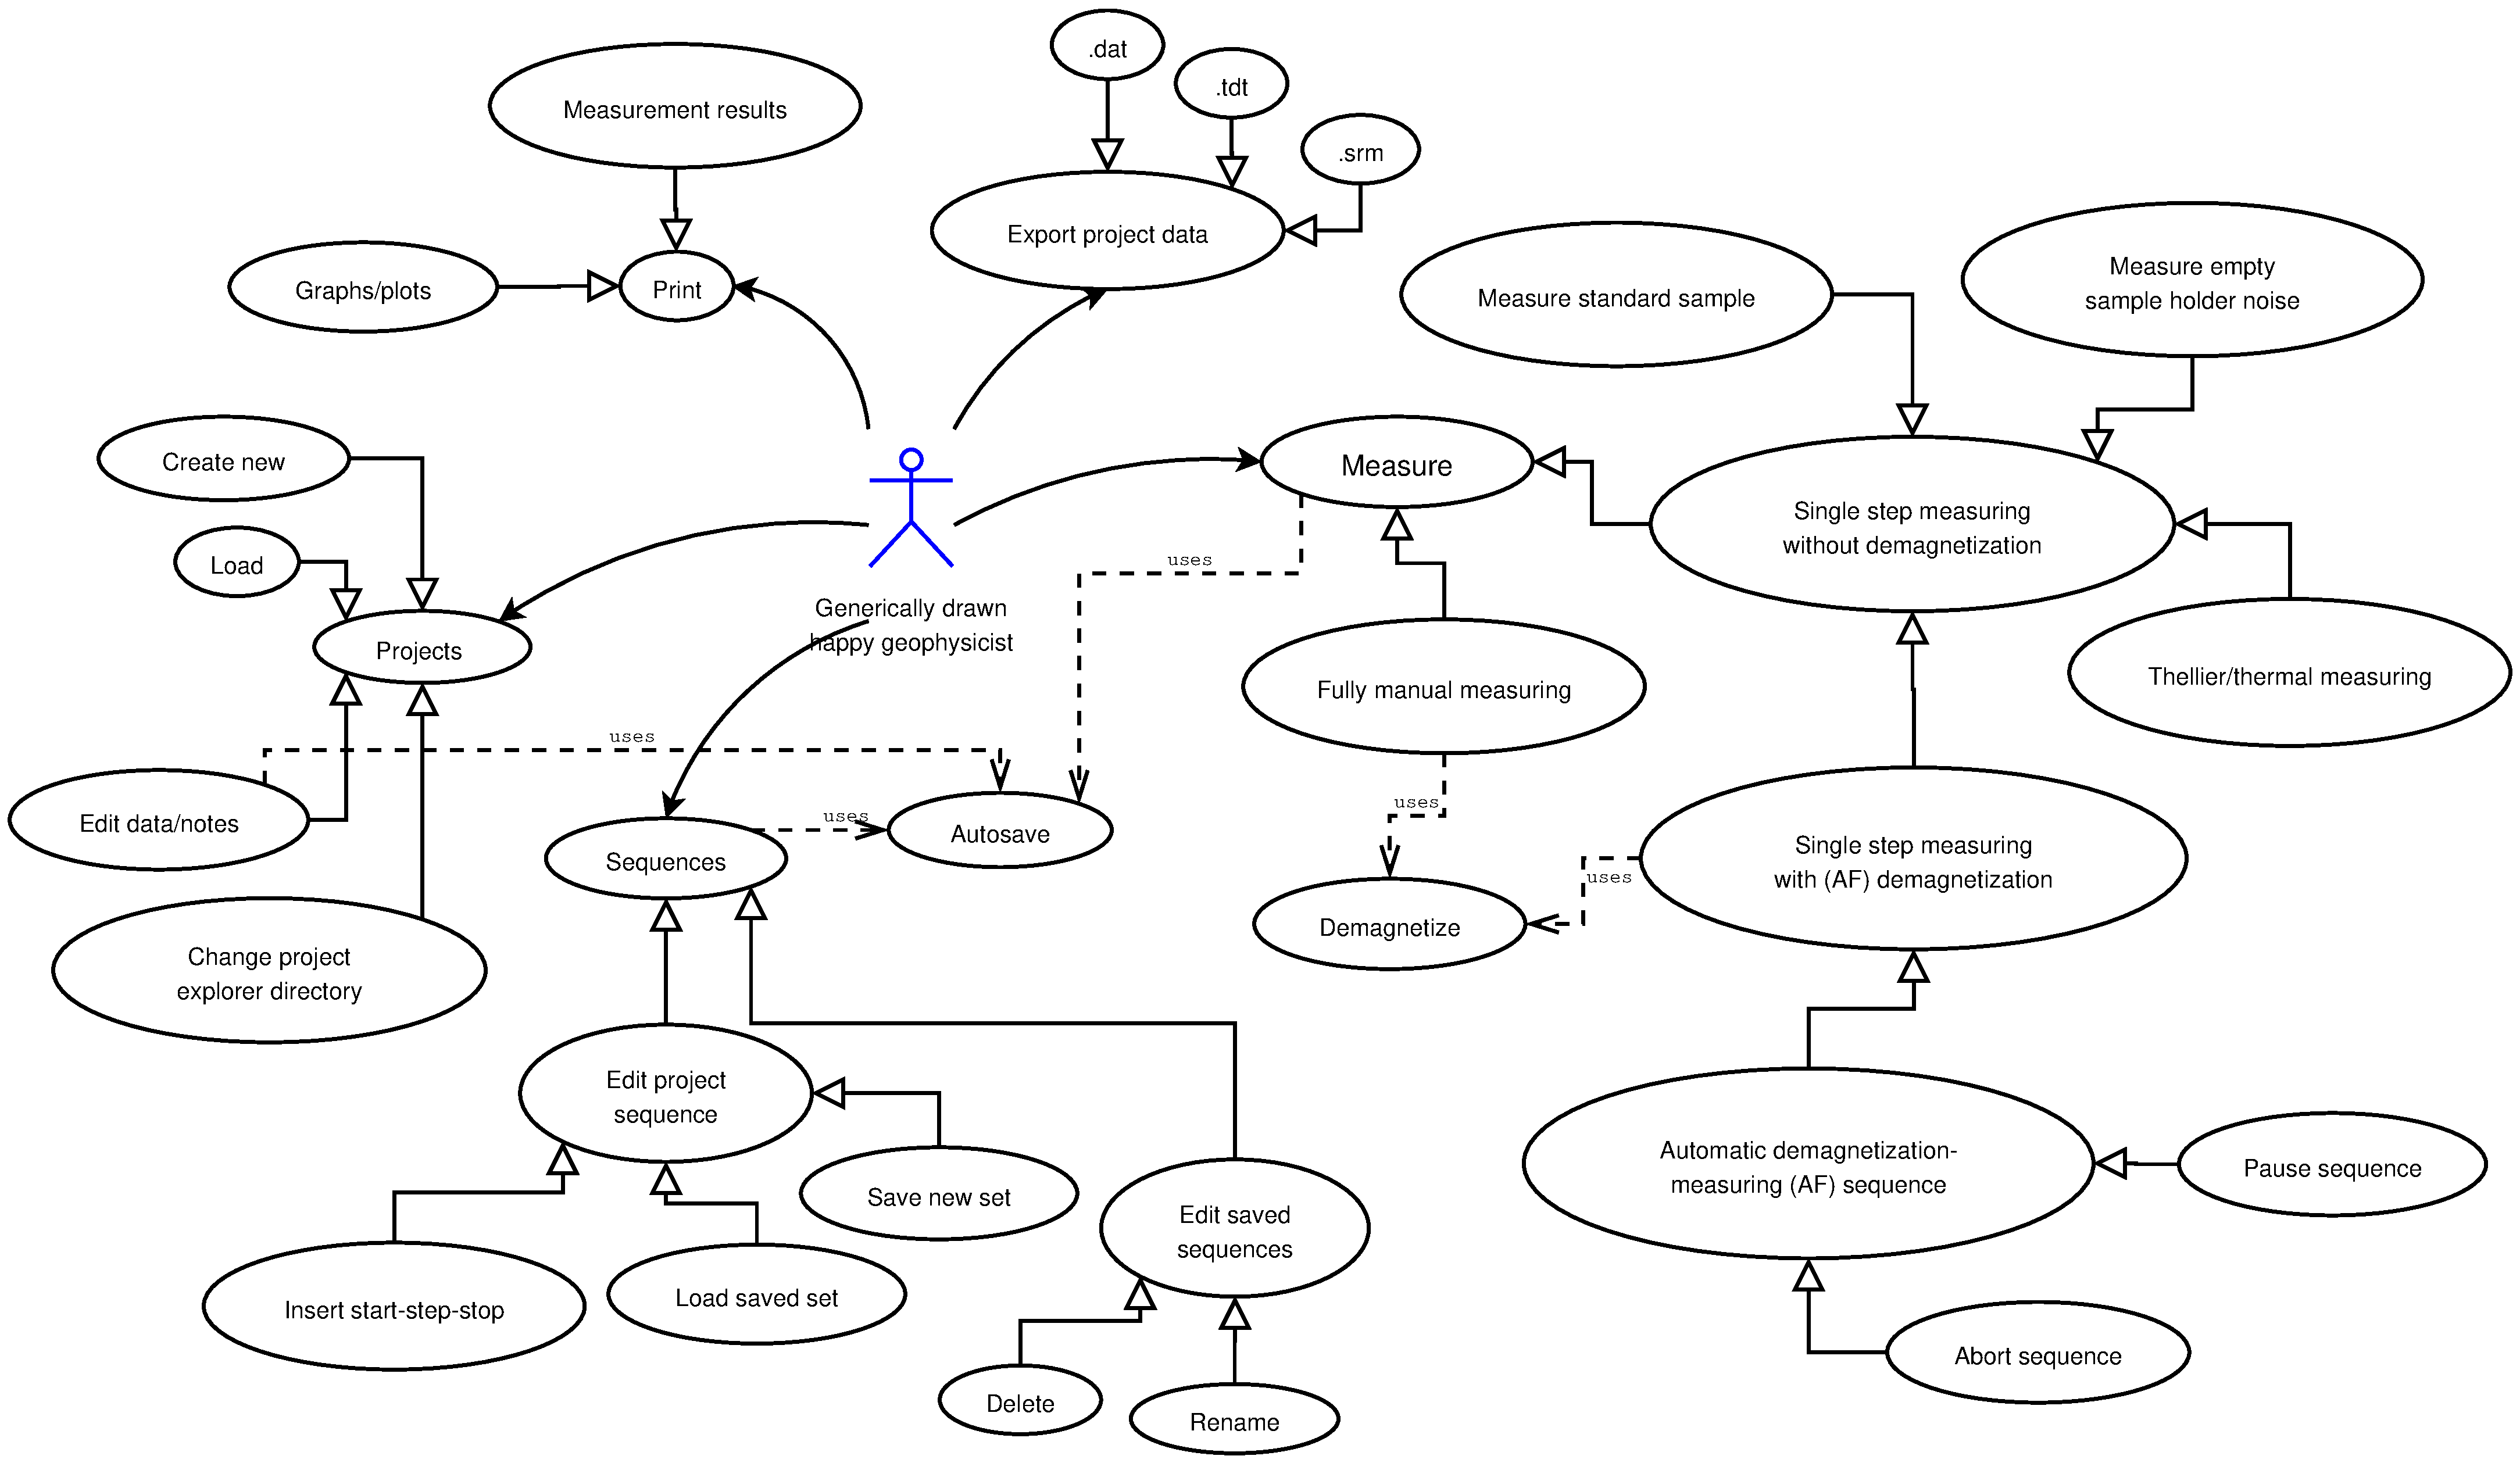
\includegraphics[angle=270,width=13cm]{usecases.eps}
\caption{Use case diagram}
\label{fig:usecases}
\end{center}
\end{figure}

Use cases are divided to different sections, grouping logically similar use cases together.

Use case format:

% lopullisesta versiosta poistettavat kommentit joko 1) [], 2) \ucnote{} tai 3) \ucnotein{} sis�ll�
\setcounter{ucnum}{-1}
\uctitle{Use case identifier and title}
\ucnote{Possible temporary note here for project group; shall be removed from final version.}
\ucscenario{First scenario for doing the use case.}
\ucscenario{Second scenario for doing the use case. ...}
\ucpre{Preconditions for use case.}
\ucpost{Postconditions for use case.}
\ucerror{Error handling, mainly if anything special needs to be done.}
\ucgd{Goal-derived use case(s) in which this use case occurs (if any); see section~\ref{seq:gduc}.}
\ucreq{Requirement(s) from which this use case derives; see section~\ref{seq:req}.}
\ucend


\subsection{Measuring}
\label{seq:ucmeasuring}

\ucsecdesc{As in any and all measuring action with the squid.}

\uctitle{Single step measuring without demagnetization}
\ucscenario{Enter as next AF demagnetization step "0" or empty (default for new projects), meaning no demagnetization, and click "Single step".}
\ucpre{AF project open, sample in sample holder.}
\ucpost{Sample measured, results on screen and appended to current project.}
\ucerror{The program shall let the user know if something went wrong.}
\ucgd{\ref{seq:gduc3}, first few steps.}
\ucreq{R1, R6, R10, R14, R17, R18}
\ucend

\uctitle{Single step measuring with (AF) demagnetization}
\ucscenario{Enter as next AF demag step anything greater than zero, and click "Single step".}
\ucpre{AF project open, sample in sample holder.}
\ucpost{Sample demagnetized (possibly ruined) and measured, results on screen and appended to current project.}
\ucerror{The program shall let the user know if something went wrong, and, should the demagnetization field not be coming down, warn user with an alarm sound :)}
\ucreq{R1, R4, R6, R10, R14, R17, R18}
\ucend

\uctitle{Automatic demagnetization-measuring sequence (AF sequence)}
\ucscenario{Enter the AF sequence (see section~\ref{seq:ucseq} for ways to enter it) and click "Measure".}
\ucpre{AF project open, sample in sample holder.}
\ucpost{Sample demagnetized according to entered AF sequence (possibly ruined) and measured after each demagnetization, results on screen and appended to current project.}
\ucerror{The program shall let the user know if something went wrong, and, should the demagnetization field be uncalm, warn user with an alarm sound x)}
\ucgd{\ref{seq:gduc1} whole sequence, \ref{seq:gduc3} sequence after few single steps at the beginning.}
\ucreq{R1, R4, R6, R10, R13, R17, R18}
\ucend
\label{uc:autoseq}

  \uctitle{Pause automatic measuring sequence}
  \ucscenario{While measure sequence is running, click "Pause".}
  \ucpre{Ongoing measuring sequence (UC\ref{uc:autoseq}).}
  \ucpost{Measure sequence halts after current step is done, results on screen.}
  \ucerror{Program tells if sequence can't be paused (and something has gone terribly wrong).}
  \ucgd{\ref{seq:gduc3}, Tomas pauses the sequence as the meteor demagnetizes too rapidly.}
  \ucreq{R1, R15}
  \ucend

  \uctitle{Abort automatic measuring sequence}
  \ucscenario{While measure sequence is running or paused, click "Stop now!".}
  \ucpre{Ongoing or paused measuring sequence (UC\ref{uc:autoseq}).}
  \ucpost{Measure sequence halts immediately \ucnotein{and program enters "fully manual" mode?}}
  \ucerror{Program tells if sequence can't be aborted (and something has gone terribly wrong).}
  \ucreq{R1, R16}
  \ucend

\uctitle{Thellier measuring}
\ucscenario{Click "Single step". (Temperature can be entered later, as it won't affect measuring.)}
\ucpre{TH project open, sample in sample holder.}
\ucpost{Sample measured, results on screen and appended to current project.}
\ucerror{As usual.}
\ucgd{\ref{seq:gduc2}, temperatures already entered, one step at 380 �C.}
\ucreq{R1, R6, R10, R14, R17, R18}
\ucend

\uctitle{Thermal measuring}
\ucnote{Exactly the same as thellier?}
\ucscenario{Click "Single step". (Temperature can be entered later, as it won't affect measuring.)}
\ucpre{TH project open, sample in sample holder.}
\ucpost{Sample measured, results on screen and appended to current project.}
\ucerror{As usual.}
\ucreq{R1, R6, R10, R14, R17, R18}
\ucend

\uctitle{Measure magnetometer ground noise}
\ucnote{2005-02-23 not in current UI proto, nor planned for implementation.}
\ucscenario{Click "Ground noise" and "Calibrate".}
\ucpre{No ongoing measurements.}
\ucpost{Ground noise measured, results on screen and appended to "Ground noise" project.}
\ucreq{R1, R3, R6, R17, R18}
\ucend

\uctitle{Measure empty sample holder noise}
\ucscenario{Click "Holder noise" and "Calibrate".}
\ucpre{No ongoing measurements, empty sample holder.}
\ucpost{Holder noise measured, results on screen and appended to "Holder noise" project.}
\ucgd{\ref{seq:gduc1}, calibration at the beginning.}
\ucreq{R1, R3, R6, R17, R18}
\ucend

\uctitle{Measure standard sample}
\ucscenario{Click "Standard sample" and "Calibrate".}
\ucpre{No ongoing measurements, standard sample in sample holder.}
\ucpost{Standard sample measured, results on screen and appended to "Standard sample" project, and, predefined .std file.}
\ucpost{Holder noise measured, results on screen and appended to "Standard sample" project.}
\ucreq{R1, R3, R6, R17, R18}
\ucend

\uctitle{Fully manual measuring}
\ucnote{2005-02-25 still not clear how fully manual is supposed to work; Tomas will be back on tuesday 1.3. and might tell us.}
\ucscenario{Click any of the manual control components.}
\ucpre{Manual mode enabled.}
\ucpost{Manual action done, result on screen \ucnotein{and appended to current project? draw graphplots?}.}
\ucreq{R1, R2, R6, R10, R17, R18}
\ucend

\uctitle{Enable manual mode}
\ucscenario{Click "Manual" checkbox above the manual control components.}
\ucpre{No ongoing measurement.}
\ucpost{Manual mode enabled.}
\ucreq{R2}
\ucend


\subsection{Exporting}
\label{seq:ucexport}

\ucsecdesc{As in exporting measurement results to another file format for othrer programs to use.}

\uctitle{Export project data into .dat file}
\ucscenario{In project explorer file list, right-click on desired project file, click "Export .dat in current directory".}
\ucscenario{In project explorer file list, right-click on desired project file, click "Export .dat to disk drive A:".}
\ucscenario{In project explorer file list, right-click on desired project file, click "Export .dat...", chooce directory and filename to export.}
\ucscenario{In project explorer file list, select multiple files with shift-click and ctrl-click, and make any of above actions.}
\ucpre{At least 1 project file in current (selected) directory.}
\ucpost{Project data exported to .dat file.}
\ucerror{Notify if file error occurs (such as no disk in A: drive).}
\ucreq{R11}
\ucend

\uctitle{Export (thellier) project data into .tdt file}
\ucscenario{In project explorer file list, right-click on desired project file, click "Export .tdt in current directory".}
\ucscenario{In project explorer file list, right-click on desired project file, click "Export .tdt to disk drive A:".}
\ucscenario{In project explorer file list, right-click on desired project file, click "Export .tdt...", chooce directory and filename to export.}
\ucscenario{In project explorer file list, select multiple files with shift-click and ctrl-click, and make any of above actions.}
\ucpre{At least 1 project file in current (selected) directory.}
\ucpost{Project data exported to .tdt file.}
\ucerror{Notify if file error occurs (such as no disk in A: drive).}
\ucreq{R11}
\ucend

\uctitle{Export single measurement details into .srm file}
\ucscenario{In measurement result table, right-click on desired measurement line(s), click "Export .srm in current directory".}
\ucscenario{In measurement result table, right-click on desired measurement line(s), click "Export .srm to disk drive A:".}
\ucscenario{In measurement result table, right-click on desired measurement line(s), click "Export...", chooce directory and filename to export.}
\ucscenario{In measurement result table, select multiple lines with shift-click and ctrl-click, and make any of above actions.}
\ucpre{At least 1 measurement result in current project.}
\ucpost{Measurement details exported to .srm file.}
\ucerror{Notify if file error occurs (such as no disk in A: drive).}
\ucreq{R11}
\ucend


\subsection{Printing}
\label{seq:ucprint}

\ucsecdesc{As in printing measurement results as text or graphs.}
\ucnotein{2005-02-25 not in current UI prototype, implementation priority low.}

\uctitle{Print measurement results}
\ucscenario{Click "Print...", "Measurement results".}
\ucpre{Open project.}
\ucpost{Measurement results printed via [Java] standard printing window.}
\ucerror{Let know if printing error occurs.}
\ucreq{R17}
\ucend

\uctitle{Print graph sheet (with 7 different graphs; described elsewhere)}
\ucscenario{Click "Print...", "Grap sheet".}
\ucpre{Open project.}
\ucpost{Measurement results printed via [Java] standard printing window.}
\ucerror{Let know if printing error occurs.}
\ucreq{R18}
\ucend


\subsection{Projects}
\label{seq:ucproject}

\ucsecdesc{As in project files, which store all measurement results.}

\uctitle{Automatically save all measurement cycles in project file}
\ucscenario{Make any measurement action (see section~\ref{seq:ucmeasuring} for those).}
\ucpre{Project file open.}
\ucpost{After measurement (step) is done, new results appended to project file.}
\ucgd{\ref{seq:gduc1}, \ref{seq:gduc2}, \ref{seq:gduc3}.}
\ucreq{R6, R10}
\ucend

\uctitle{Create new project}
\ucscenario{Click the empty line below filenames in project explorer, enter new project name, chooce AF/TH (thellier) project, click "Create new" or press enter.}
\ucpre{Project explorer in desired directory (UC\ref{uc:choosedir}).}
\ucpost{New project created and selected.}
\ucgd{\ref{seq:gduc1} after calibration, \ref{seq:gduc3} at the beginning.}
\ucreq{R5}
\ucend

\uctitle{Load project}
\ucscenario{Click any filename in project explorer.}
\ucpre{Project explorer in desired directory (UC\ref{uc:choosedir}). A measurement can be running at the same time (it will be highlighted in the project explorer).}
\ucpost{Existing project loaded and selected.}
\ucgd{\ref{seq:gduc2} all samples already as project files.}
\ucreq{R7, R10}
\ucend

\uctitle{Change project explorer directory}
\ucscenario{Click into current directory textbox in project explorer, write directory to change to. If the typed directory exists, the program will open it automatically. \ucnotein{Or will a push of Enter be anyway required to change directory? Should we try both before deciding?}}
\ucscenario{Click into current directory textbox in project explorer, start writing directory; when autocomplete-results appear below, use up/down+enter or mouseclick to select the directory.}
\ucscenario{Click the down-arrow on the right side of current directory textbox in project explorer, choose desired directory from appearing directory history.}
\ucscenario{Click "Browse..." in project explorer, use standard [Java] file chooser to select directory to change to.}
\ucpre{There is no measurement running right now (to prevent the user from getting lost).}
\ucpost{The contents of the chosen directory are shown in the project explorer. The newest project file in the directory will be selected and loaded.}
\ucerror{If the user has typed an invalid directory, then a "No such directory" message will be displayed in place of the autocomplete-results.}
\ucgd{\ref{seq:gduc1}, \ref{seq:gduc2}, \ref{seq:gduc3}.}
\ucend
\label{uc:choosedir}

\uctitle{Insert/edit project data}
\ucscenario{Click any of the project data checkboxes, or textboxes and enter value.}
\ucpre{Project file open (usually just created it).}
\ucpost{Project data changed, measuring results recalculated, saved automatically to project file. Saving can happen after a short delay to avoid unnecessary file system access.}
\ucgd{\ref{seq:gduc1} after creating new project.}
\ucreq{R6, R8, R9}
\ucend


\subsection{Sequences}
\label{seq:ucseq}

\ucsecdesc{As in automatic demagnetization-measuring sequences (AF sequences), or, thellier temperature sequences.}

\uctitle{Insert sequence manually}
\ucscenario{Click "Tesla" or "Temp" column in the last line (which is empty) of measurement result table, enter value; press down, [tab?] or enter to advance to a new line, enter value; and so on.}
\ucpre{An open project.}
\ucpost{Sequence appended to measurement result table and current project.}
\ucgd{\ref{seq:gduc3} after creating new project.}
\ucreq{R6, R12}
\ucend

\uctitle{Insert sequence with start-step-stop values}
\ucscenario{Click "Start" textfield, insert start value (default value is the last value of the Tesla/Temp column), click "Step" textfield, insert step value, click "Stop" textfield, insert stop value, click "Add sequence" or press enter.}
\ucscenario{Click "Start" textfield, insert start value (default value is the last value of the Tesla/Temp column), press tab, insert step value, press tab, insert stop value, press enter or click "Add sequence".}
\ucpre{An open project.}
\ucpost{Sequence from {\it start} to {\it stop}, increasing by {\it step} for every step, appended to measurement result table of the current project. Value of "Start" textfield is the previous value of "Stop". "Step" and "Stop" textfields are empty. "Step" textfield has focus.}
\ucerror{If the last value in the old sequence (excluding completed measurements) is equal to the {\it start} value of this new sequence, then start the new sequence from {\it start + step}.}
\ucgd{\ref{seq:gduc3} after creating new project and entering manual values.}
\ucreq{R6, R12}
\ucend

\uctitle{Load sequence}
\ucscenario{Click down-arrow in right side of "Load set" combo box; from appearing list, click sequence to load.}
\ucpre{An open project, at least 1 saved sequence.}
\ucpost{Selected sequence appended and selected to measurement result table, and appended to current project.}
\ucgd{\ref{seq:gduc1}, after typing project data, load "Basalt" set; \ref{seq:gduc2} set already loaded for each project file (when created).}
\ucreq{R6}
\ucend
\label{uc:loadseq}

\uctitle{Edit sequence on-the-fly}
\ucscenario{Click any unmeasured "Tesla" or "Temp" column in measurement result table, enter new value.}
\ucscenario{Click any unmeasured line in measurement result table, press del to delete that line.}
\ucscenario{Right-click any unmeasured line in measurement result table, choose "Delete" to delete that line.}
\ucscenario{Click-drag any unmeasured line in measurement result table to new position within unmeasured lines.}
\ucscenario{Select multiple unmeasured lines in measurement result table with shift-clicks and ctrl-clicks, make any of above actions (except enter new value).}
\ucpre{Unmeasured lines in current project's measurement result table (note that measuring sequence can be going on).}
\ucpost{Editing committed, saved to current project.}
\ucerror{Editing or screwing up measured lines won't be allowed.}
\ucgd{\ref{seq:gduc3}, when sequence demagnetizes too rapidly, Tomas deletes unmeasured lines.}
\ucreq{R6}
\ucend
\label{uc:editseq}

\uctitle{Save sequence}
\ucscenario{Click "Load set" combo box, enter new sequence name, click "Save set". \ucnotein{2005-02-25 not in current (almost final) UI prototype!}}
\ucscenario{Right-click any line in measurement result table, choose "Save full sequence...", enter name, press enter.}
\ucscenario{Select any lines in measurement result table with shift-clicks and ctrl-clicks, right-click on selected lines, choose "Save selected sequence...", enter name, press enter.}
\ucpre{At least 1 line in measurement results table (although you propably don't want to save a sequence with only one step x).}
\ucpost{New sequence set saved to predefined sequence file and available from "Load set" combo box.}
\ucerror{Ask whether to overwrite, if sequence with the same name already exists (allow to enter new name if choose not to overwrite).}
\ucend
\label{uc:saveseq}

\uctitle{Edit stored sequence}
\ucscenario{UC\ref{uc:loadseq} "Load sequence" -> UC\ref{uc:editseq} "Edit sequence" -> UC\ref{uc:saveseq} "Save sequence" with same name as the loaded sequence.}
\ucscenario{Click menu "Options"->"Sequences...", edit any sequence in appearing window... \ucnotein{2005-02-25 not in UI prototype, must be improvised :)}}
\ucpre{At least 1 saved sequence.}
\ucpost{Changes saved to predefined sequence file.}
\ucend

\uctitle{Delete stored sequence}
\ucscenario{Click down-arrow in right side of "Load set" combo box; from appearing list, right-click sequence to delete, choose "Delete".}
\ucscenario{Click menu "Options"->"Sequences...", delete sequence in appearing window... \ucnotein{2005-02-25 not in UI prototype, must be improvised :)}}
\ucpre{At least 1 saved sequence.}
\ucpost{Sequence deleted, changes saved to predefined sequence file.}
\ucend

\uctitle{Rename stored sequence}
\ucscenario{Click down-arrow in right side of "Load set" combo box; from appearing list, right-click sequence to rename, choose "Rename...", enter new name, press enter.}
\ucscenario{Click menu "Options"->"Sequences...", rename any sequence in appearing window... \ucnotein{2005-02-25 not in UI prototype, must be improvised :)}}
\ucpre{At least 1 saved sequence.}
\ucpost{Sequence renamed, changes saved to predefined sequence file.}
\ucend



\section{Requirements}
\label{seq:req}

% Makrot vaatimuksille
\newcommand{\ReqId}[1]{\textbf{Identifier:} #1\\}
\newcommand{\ReqName}[1]{\textbf{Name:} #1\\}
\newcommand{\ReqDesc}[1]{\textbf{Description:} #1\\}
\newcommand{\ReqPrio}[1]{\textbf{Priority:} #1\\}
\newcommand{\ReqSet}[1]{\textbf{Set by:} #1\\}
\newcommand{\ReqUc}[1]{\textbf{Use Cases:} #1\\}

Goals of the software set by client, project team and environment.
Requirements were collected from 1) powerpoint slides received from
client, 2) lectures given by client, 3) user observations held at the
squid lab with client (used to collect goal-derived use cases), and 4)
user interface prototype demonstrations given to client, after which the
client gave suggestions and corrections to prototype functions.

Priorities are from 1 (highest) to 4 (lowest). Our goal is to fulfill at
least the requirements with priorities 1 and 2. Requirements with
priority 3 will be fulfilled only if time permits, and priority 4's will
propably be left out.

\ReqId{Requirements identifier}
\ReqName{Name of the requirement}
\ReqDesc{Description of the requirement.}
\ReqPrio{Requirements priority from 1(most important) to 4(least important)}
\ReqSet{Who set the requirement}
\ReqUc{Use cases derived from the requirement}


\subsection{Functional requirements}

Define the services which the software offers and how the software behaves, including error handling. May also define things the software shall not do.

\subsubsection{Magnetometer}

\ReqId{R1}
\ReqName{SQUID control and usage}
\ReqDesc{Able to control Squid-magnetometer and make measurements with it.}
\ReqPrio{1}
\ReqSet{Customer}
\ReqUc{UC1, UC2, UC3, UC4, UC5, UC6, UC7, UC8, UC9, UC10, UC11}

\ReqId{R2}
\ReqName{Manual control}
\ReqDesc{Able to operate the magnetometer manually. User can move and
rotate sample handler and measure and demagnetize sample.}
\ReqPrio{3}
\ReqSet{Customer}
\ReqUc{UC11, UC12}

\ReqId{R3}
\ReqName{Calibration reminder}
\ReqDesc{Magnetometer must be calibrated every 24 hours. The program will remind the user when it would be time to do calibration.}
\ReqPrio{2}
\ReqSet{Customer}
\ReqUc{UC8, UC9, UC10}

\ReqId{R4}
\ReqName{Warning signal}
\ReqDesc{Program should warn user with alarm signal if magnetic field
remains on for too long.}
\ReqPrio{1}
\ReqSet{Customer}
\ReqUc{UC2, UC3}


\subsubsection{Project files}

\ReqId{R5}
\ReqName{Create project}
\ReqDesc{Create a new project file which will include the measurement sequence, measurement results and information about the sample. The file format will be custom made for this program.}
\ReqPrio{1}
\ReqSet{Customer}
\ReqUc{UC19}

\ReqId{R6}
\ReqName{Autosave project}
\ReqDesc{Program will save measurement data and project information after every measurement step and modification.}
\ReqPrio{1}
\ReqSet{Customer}
\ReqUc{UC1, UC2, UC3, UC6, UC7, UC8, UC9, UC10, UC11, UC18, UC22, UC23,
UC24, UC25, UC26}

\ReqId{R7}
\ReqName{Load project}
\ReqDesc{Saved projects can be loaded into program.}
\ReqPrio{1}
\ReqSet{Customer}
\ReqUc{UC20}

\ReqId{R8}
\ReqName{Edit project}
\ReqDesc{Ability edit project information and measurement data afterwards. (TODO: which data fields?)}
\ReqPrio{2}
\ReqSet{Customer}
\ReqUc{UC22}

\ReqId{R9}
\ReqName{Recalculate derived measurement data}
\ReqDesc{When the measurement data or the mass/volume of the specimen is changed, recalculate all numbers that have been derived from the modified data.}
\ReqPrio{2}
\ReqSet{Customer}
\ReqUc{UC22}

\ReqId{R10}
\ReqName{Append project}
\ReqDesc{New measurements can be added to existing projects.}
\ReqPrio{2}
\ReqSet{Customer}
\ReqUc{UC1, UC2, UC3, UC6, UC7, UC11, UC18, UC20}

\ReqId{R11}
\ReqName{Export to other file formats}
\ReqDesc{Measurements can be saved in .dat, .tdt and .srm files.}
\ReqPrio{1}
\ReqSet{Customer}
\ReqUc{UC13, UC14, UC15}


\subsubsection{Measurements}

\ReqId{R12}
\ReqName{Create a measurement sequence}
\ReqDesc{Able to create AF and Thellier measurement sequences with several different sized steps.}
\ReqPrio{2}
\ReqSet{Customer}
\ReqUc{UC23, UC24}

\ReqId{R13}
\ReqName{Automatic sequence}
\ReqDesc{Do all the measurement steps automatically.}
\ReqPrio{2}
\ReqSet{Customer}
\ReqUc{UC3}

\ReqId{R14}
\ReqName{Single step sequence}
\ReqDesc{Do only one measurement step at a time.}
\ReqPrio{2}
\ReqSet{Customer}
\ReqUc{UC1, UC2, UC6, UC7}

\ReqId{R15}
\ReqName{Pause automatic sequence}
\ReqDesc{Able to stop the measurement sequence after current step. After being stopped, the user can make modifications to the sequence and continue from where the sequence was left.}
\ReqPrio{2}
\ReqSet{Customer}
\ReqUc{UC4}

\ReqId{R16}
\ReqName{Panic abort}
\ReqDesc{Able to stop any measurement immediately. The demagnetizer will be turned off and the sample holder will stop where it is. The current measurement data will be discarded.}
\ReqPrio{1}
\ReqSet{Customer}
\ReqUc{UC5}

\ReqId{R17}
\ReqName{Numeric presentation of measurements}
\ReqDesc{Program shows measurement data in numbers. Measurement data will be displayed using scientic notation (1.23e4).}
\ReqPrio{1}
\ReqSet{Customer}
\ReqUc{UC1, UC2, UC3, UC6, UC7, UC8, UC9, UC10, UC11, UC16}

\ReqId{R18}
\ReqName{Graphic presentation of measurements}
\ReqDesc{Program draws graphs from measurement data. Available graph types are: Stereo Plot, Intensity, Zijderveld, Difference Vectors, Susteptibility, O63, Great Circles. (TODO: what are the definitions of these graphs? priorities per graph?)}
\ReqPrio{4}
\ReqSet{Customer}
\ReqUc{UC1, UC2, UC3, UC6, UC7, UC8, UC9, UC10, UC11, UC17}


\subsubsection{Others}

\ReqId{R19}
\ReqName{Hotkeys}
\ReqDesc{The program has hotkeys for the most often used operations.}
\ReqPrio{3}
\ReqSet{Customer}

\ReqId{R20}
\ReqName{Change hotkeys}
\ReqDesc{Possibility to change hotkey assignments.}
\ReqPrio{4}
\ReqSet{Customer}


\subsection{Quality requirements}

\ReqId{QR1}
\ReqName{Error free}
\ReqDesc{The program should not crash. All the functions need to work as documented. The calculations that the program makes from measurements must be done right.}
\ReqPrio{1}
\ReqSet{Customer}

\ReqId{QR2}
\ReqName{Ease of use}
\ReqDesc{Program should be easy to use for first time users after it has been explained to them how to take measurements with the magnetometer.}
\ReqPrio{1}
\ReqSet{Customer}

\ReqId{QR3}
\ReqName{Quality of documentation}
\ReqDesc{The documentation must be so good that other teams can easily continue the development. Program should have good help pages for the end-users.}
\ReqPrio{2}
\ReqSet{Group}

\ReqId{QR4}
\ReqName{Performance}
\ReqDesc{The program must keep up with the SQUID hardware. The user interface should not freeze for periods of over 0,5 seconds.}
\ReqPrio{2}
\ReqSet{Group}

\ReqId{QR5}
\ReqName{Expandable architecture}
\ReqDesc{It should be possible to expand the program to process the measurement data in more ways.}
\ReqPrio{2}
\ReqSet{Group}


\subsection{Environment}

{\it Define requirements for the software which origin from the environment
in which the sowtware will be working, and which the software must satisfy for 
being able to work in its environment.}

Program will be used in normal PC which is connected to magnetometer. The 
computer that will run this program will be equal or better to 1GHz CPU, 256MB 
RAM, 1280x1024 resolution. The current computer is running Windows XP.

Taking into account rapid phase of computer evolution it is possible that 
computer in which program is used can change, accordingly the program should be 
installable by outsiders. We need not prepare to changing of magnetometer, as 
new magnenetometer will probably have its own program. Program doesn't
control temparature of magnetometer.

The SQUID hardware and communication with it is described in the section 
"External interfaces".


\subsection{Maintainability}

It must be possible to continue the development of the program. The 
documentation must be complete so that other teams can quickly continue the 
development even if they have not studied user interface designing. It must be 
possible to add new graph types to the program and export the measurement data 
to other programs.



\section{User interface}

Overview of UI described here.. 

\subsection{Goal-derived use cases}
\label{seq:gduc}

\subsubsection{Goal-derived use case 1: Erkki...}
\label{seq:gduc1}

\subsubsection{Goal-derived use case 2: Fabio...}
\label{seq:gduc2}

\subsubsection{Goal-derived use case 3: Tomas...}
\label{seq:gduc3}



\section{Architecture overview}

The program architecture can be divided into three parts: SQUID interface, 
measurement project and user interface. The program will also communicate with 
the SQUID hardware and local file system. A graphical representation of the 
architecture can be seen in Figure~\ref{fig:architecture}.

\begin{figure}
\begin{center}
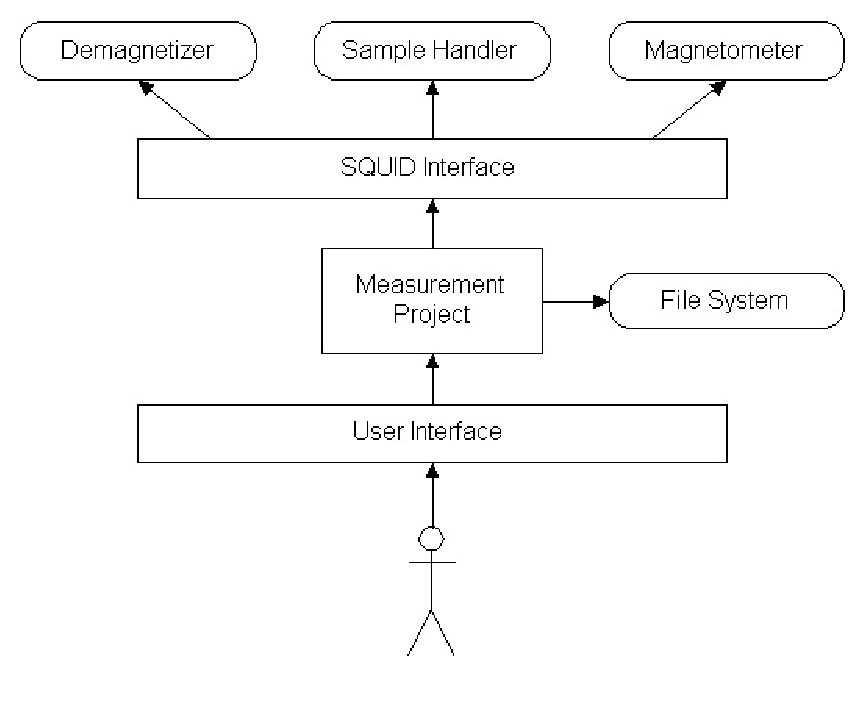
\includegraphics[width=10cm]{architecture.eps}
\caption{Architecture overview}
\label{fig:architecture}
\end{center}
\end{figure}

SQUID interface is responsible for controlling the hardware in an orderly 
manner. It will provide high- and low-level controls for using the hardware. 
Communication with the hardware is done via COM ports. The SQUID interface will 
hide the protocol-level commands from the programmer and prevent illegal use of 
the hardware.

Measurement project is responsible for managing the project information, 
measurement sequence and measurement data. It will recieve commands from the 
user interface and notify the UI when the state of the project changes. It will 
send commands to the SQUID interface, recieve measurement data and save it. When 
the internal data of the project changes, the copy on the local file system will 
be automatically synchronized after a short delay (1 second or less).

User interface is responsible for communicating with the user of the program. It 
will update itself whenever the state of the measurement project is changed. It 
will send commands from the user to the program.



\section{External interfaces}

Interfaces to existing software and hardware are described here.

\subsection{Existing program}

The existing software for using the SQUID is "2G Enterprises Data Acquisition". 
We have access to the source code for version 2.99.3 of the program. From the 
old source code we will reuse basically only the SerialIO component. We will 
build an interface for communicating with the SQUID hardware by using Java and 
JNI (Java Native Interface).

\subsection{Hardware control protocols}

The SQUID consists of three independent units:

\begin{itemize}
\item Automated Sample Handler System (MODEL 2G800)
\item Automatic Sample Degaussing System (MODEL 2G600)
\item Superconducting Rock Magnetometer (MODEL 755R or 760R)
\end{itemize}

Automated Sample Handler System controls the movement and rotation of the sample 
holder. Its protocol is described in Appendix 1.

Automatic Sample Degaussing System controls the demagnetizer. Its protocol is 
described in Appendix 2.

Superconducting Rock Magnetometer reads the measurements from the magnetometer. 
Its protocol is described in Appendix 3.



\section{Validation}

In validation it is shown that program meets requirements set by user.
Project documents are validated in reviews. Program code is validated by
testing. In reviews it will be established that requirement document and
design document are in line with user requirements and will lead
to production of program which meets these requirements. Testing shows
that program actually works as specified by design document.
